\documentclass[tikz,border=8pt]{standalone}
\usepackage{amsmath}
\usetikzlibrary{decorations.markings}
\usetikzlibrary{arrows.meta,calc,angles,quotes}
\usetikzlibrary{external}

% -------------------------------------------------
% Custom PGF/TikZ shape based on the supplied path
% -------------------------------------------------
\makeatletter
\pgfdeclareshape{wing}{
	
	% Standard anchors
	\savedanchor\centerpoint{\pgfpoint{0}{0}}
	
	\anchor{center}{\centerpoint}
	\anchor{north}{\pgfpoint{0}{1.7cm}}
	\anchor{south}{\pgfpoint{0}{-1.5cm}}
	\anchor{west}{\pgfpoint{-8cm}{0}}
	\anchor{east}{\pgfpoint{0}{0}}
	
	% Recommended text box
	\foregroundpath{
		% Scale down to resemble original drawing
		\pgftransformscale{0.5}
		
		\pgfpathmoveto{\pgfpoint{0cm}{0cm}}
		
		\pgfpathcurveto
		{\pgfpoint{-1.8cm}{0.9cm}}
		{\pgfpoint{-5.5cm}{1.7cm}}
		{\pgfpoint{-8cm}{0.25cm}}
		
		\pgfpathcurveto
		{\pgfpoint{-9cm}{-0.35cm}}
		{\pgfpoint{-8.2cm}{-1.5cm}}
		{\pgfpoint{-6.2cm}{-1.05cm}}
		
		\pgfpathcurveto
		{\pgfpoint{-3.8cm}{-0.55cm}}
		{\pgfpoint{-1.4cm}{0.2cm}}
		{\pgfpoint{0cm}{0cm}}
		
		\pgfpathclose
		
		\pgfsetlinewidth{0.8pt}
		\pgfsetstrokecolor{blue}
		\pgfusepath{draw}
	}
}
\makeatother

\tikzexternalenable

\begin{document}
	
	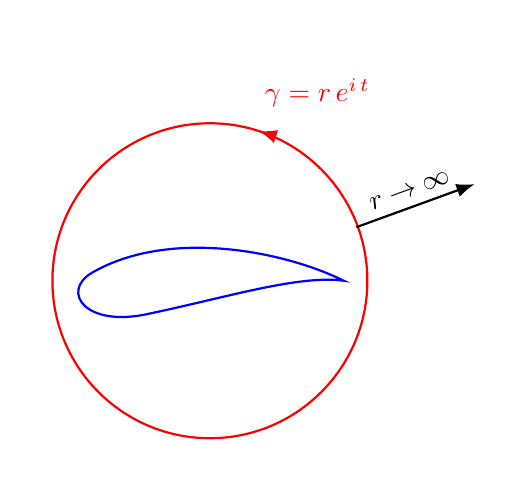
\begin{tikzpicture}[scale=0.4,>=Latex]
		\coordinate (P) at (0,4.7);
		\draw[white, thick] (-10,-6) rectangle (5,8);
		\node[shape=wing, scale = 0.8] at (0,0) {};
		
		\draw[thick, red,
		postaction={
			decorate,
			decoration={
				markings,
				mark=at position 0.2 with {\arrow{Latex}}
			}
		}]
		(-4.25,0) circle (5);
		
		\node [above, text width=2cm, align=left, minimum height=1cm] at (P) {\color{red}$\gamma = r \, e^{i \, t}$};
		
		\draw[->, thick, black] (0.4, 1.7) -- node [sloped, midway, above] {$r \rightarrow \infty$} + (20:4);
	\end{tikzpicture}
	
\end{document}